\documentclass[notitlepage]{article}
\usepackage{lmodern}
\usepackage{tikz}
\usetikzlibrary{automata,positioning}
\usepackage{enumitem}
\usepackage{amsmath}
\usepackage{enumitem}
\usepackage{cancel}
\usepackage{stackengine}
\usepackage{hyperref}
\usepackage{subfig}


\def\delequal{\mathrel{\ensurestackMath{\stackon[1pt]{=}{\scriptstyle\Delta}}}}
\title{Plasmodium fulciparum Vaccine Immunogenicity}
\author{Ahmad Shayaan IMT2014004 \\ Indu Ilanchezian IMT2014024}
\def\dotminus{\mathbin{\ooalign{\hss\raise1ex\hbox{.}\hss\cr \mathsurround=0pt$-$}}}


\begin{document}
	\maketitle
	\pagenumbering{gobble}
	\pagenumbering{arabic}
	
	\section{Introduction}
	Malaria is a life-threatening disease caused by parasites that are transmitted to the human hosts by the female Anopheles mosquitoes \cite{item0}. Around 3.2 billion people live in areas at risk of malaria transmission in 106 countries and territories \cite{item01}. Malaria is caused by five species of Plasmodium protozoa. The most deadly among the five is Plasmodium falciparum \cite{item0}. 
	Malaria is being controlled worldwide by preventive measures such as spraying insecticides or treated using antimalarial drugs. However, malaria eradication, globally, still seems to be a matter of the future. Despite decades of clinical trials and experimentation, there is no known effective vaccine against malaria till date. The most advanced vaccine is the RTS,S/ASO1 which is also in the Phase-3 trials \cite{item02}. Most of the other vaccine proposals are still undergoing trials. A majority of these vaccines are subunit vaccines. Subunit vaccines use the wealth of available genome sequence data of the pathogen. A portion of the organism's proteome sequence coupled with an adjuvant is used as a vaccine \cite{item6}. In our work, we aim to find out methods to reduce the time needed to measure the effectiveness of a vaccine using machine learning. We also aim to formulate machine learning models which can effectively identify the antigenic sequences from the entire genome sequence of Plasmodium falciparum. 
	
	\section{Problem Statements}
		\subsection{Predicting whether individuals vaccinated against Malaria will measurably benefit from the vaccine or not}
		Vaccine trial aims to establish the safety and efficacy of a vaccine prior to it being licensed. The vaccine is tested in different phases which are.
		\begin{enumerate}
			\item \textbf{Phase One trial} - The following stage in vaccine trials is the phase one study, which consists of introducing the drug into the human population.
			\item \textbf{Phase Two trial} - Phase two will consist of more healthy volunteers in the vaccine target population (~100s of people) to determine reactions in a more diverse set of humans and test different schedules.
			\item \textbf{Phase Three trial} - The vaccine must be shown to be safe and effective in natural disease conditions before being submitted for approval and then general production.
			\item \textbf{Phase Four trial} - Phase four trials are typically monitor stages that collect information continuously on vaccine usage, adverse effects, and long-term immunity.\cite{item1}
		\end{enumerate}
	
	Vaccine trials may take months or years to complete, since a sufficient time period must elapse for the subjects to react to the vaccine and develop the required antibodies. 
	
	Predicting whether a vaccine is successfully administered in a subject will help shorten the testing phase of the vaccine development, thus helping in making vaccine faster.
	
	\subsubsection{Dataset used}
	For predicting whether the vaccination was successful or not we needed the genetic expression data of subjects which were administered with malaria vaccine.
	
	We used the GSE18323 data set from NCBI(National Center for Biotechnology Information) which was collected by the Walter Reed Army Institute of Research
	Department.
	
	The Volunteers were assessed for the study, and the genetic responses were collected from the volunteers on the third day of the third vaccination and 24, 72 hours, two weeks after vaccination, and 5 days after challenge.\cite{item2}
	
	There were 39 subjects from which the data was collected. Out of all the 39 subjects only 13 were successfully protected by the vaccine and 26 remained unprotected.
	
	The data set was available in CEL format, which is a data file created by Affymetrix DNA microarray image analysis software. Each file consisted of 22,000 genetic entries for each subject.
	
	\subsubsection{Challenges Faced}
	 There were two significant problems that we faced during the process of solving the problem statement. They are as follows.
	 
	 \begin{enumerate}
	 	\item \textbf{Small number of samples} - The dataset consisted of only 39 data points, which not sufficient for a learning algorithm to produce a good enough model. To counter this problem we synthesized our own data by randomly selecting subjects from the existing data points, and then adding a small amount of noise to the genetic markers of the subjects.
	 	
	 	\item \textbf{Class Imbalance} - The data points that were synthesized were biased to the non protected class as the original data points had a higher number of unprotected subjects. To deal with the class imbalance we trained the model with pre-computed wights for all the classes. The weights computed were inversely proportional to the class frequency in the data.
	 \end{enumerate}
	
	\subsubsection{Experiments}
	To predict whether the subject was successfully immunized or not we trained a logistic regression model with the entire humane genome information present in the dataset.
	
	The logistic regression model was trained for each time instance separately. This was done because we wanted to find at which instance the protected and non-protected class showed the most distinguishing features.
	
	The model was trained on different data set sizes of 100, 125, 150, 200 and 600 data points. The best results were obtained for the dataset with 200 data points.
	
	\subsubsection{Results}
	
	The results obtained for different days are as follows-
	
	\begin{table}[!h]
		\centering
		\caption{Accuracies}
		\label{Accuracies}
		\resizebox{\columnwidth}{!}{%
		\begin{tabular}{|c|c|c|}
		\hline	Time Instance& Accuracy of the dataset size 150 & Accuracy of the dataset size 200 \\ 
		\hline On the day of the vaccination& \ 87\% & 95\%  \\ 
		\hline 24 hours after vaccination& 95\% & 95\% \\ 
		\hline 72 hours after vaccination& 92\% & 99\% \\ 
		\hline Two weeks after vaccination& 93\%& 95\% \\ \hline 
		\end{tabular}
	}
	\end{table}

	The best results were obtained for data set of size 200, 72 hours post vaccination.
	
	\begin{figure}[!tbp]
		\centering
			\subfloat[150 samples size, 24 hours post vaccination]{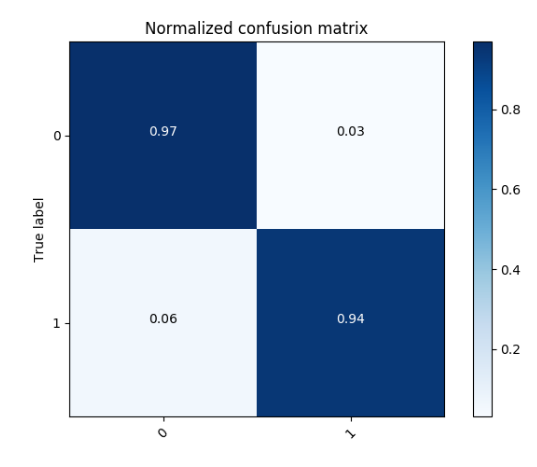
\includegraphics[width=0.4\textwidth]{img1.png}\label{fig:f1}}
		\hfill
		\subfloat[200 samples size, 72 hours post vaccination]{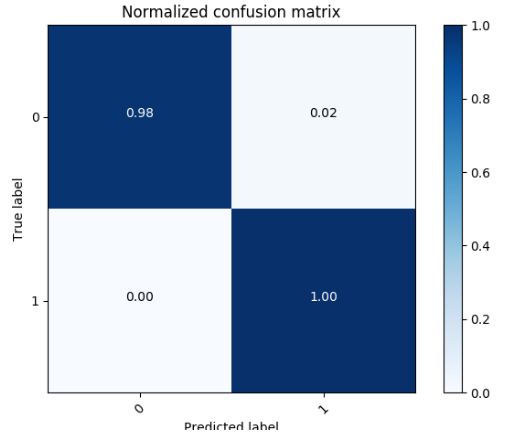
\includegraphics[width=0.4\textwidth]{img2.png}\label{fig:f2}}
		\caption{Accuracies}
	\end{figure} 
	
	\subsection{Predicting antigenic sequence from the proteome sequence of Plasmodium Falciparum}
	
	The Plasmodium Falciparum pathogen has over 6000 genes\cite{item3} predicting if the gene sequence is antigenic or not will help in making subunit vaccines. Subunit vaccine do not contain live components of the pathogen, they only introduce the antigens to the immune system to generate a response\cite{item4}.
	
	Antigen are those protein sequences which are capable of inducing an immune response in the host.
	
	
	\subsubsection{Dataset used}
	The dataset of all the proteome sequences was obtained form UniProtKB. UniProt is an open source data repository of protein sequences of various organism.
	
	The dataset contained about 120,000 protein sequences for Plasmodium Falciparum , out which only 357 protein sequences were reviewed. The length of the protein sequence varied in length from 10 to 10,000 individual proteins.
	
	The labels for the reviewed gene sequences were not present in Uniprot. We used the IEDB(Immuno Epitope Database). The sequences extracted from uniprot were associated with their labels using IEDB.
	
	\subsubsection{Feature set}
	The raw data obtained from UniProtKB is in the form of sequence of amino acids. This has to converted to numerical values in order to proceeed with training statistical models. Few properties which determine antigenicity are:
	\begin{enumerate}
	\item Hydrophobicity
	\item Flexibility
	\item $\alpha$ helix
	\item $\beta$ turns
	\item Polarity
	\item Antigen Index
	\item TFA Retention
	\item Accessibility
	\end{enumerate}\cite{item7}
	These properties of amino acids are used as features. With this step, we have converted the protein sequences to a sequence of numerical features and data is now ready to be fit with statistical models.  
	
	\subsubsection{Methods used to find antigenic sequences}
	
	\paragraph{Hidden Markov Model}.\\ \\
	Hidden Markov Models are statistical model in which the system being modeled is assumed to be a Markov chain with hidden states.
	
	The output of the underlying system are a set of observations dependent of the hidden states of the Markov chain.
	
	The Hidden Markov model can be described as a five tuple as $(S,V,\Pi,A,B)$. Where the entries of the tuple are as follows:
	
	\begin{enumerate}
		\item \textbf{S} = \{$s_1, ..., s_n$ \} It is the set of the states in the Markov chain.
		\item \textbf{V} = \{$v_1, ..., v_n$ \} It is the set of all the possible symbols in the vocabulary.
		\item \textbf{$\Pi$} = \{$\pi_i$\} It is the probability of starting the stare sequence at state i.
		\item \textbf{A} = The matrix containing all the transition probabilities.
		\item \textbf{B} The matrix of all the emission probabilities.
  	\end{enumerate}
 
  	The basic problems that HMM can be used on are
  	
  	\begin{enumerate}
 		\item \textbf{Evaluation}: Evaluating the probability of an observed sequence of symbols O = $\{o_1, o_2, ...,o_T\}$ ($o_i \in V$ ), given a particular HMM, i.e., $P(O \mid M)$
 		
 		\item\textbf{Decoding}: Finding the most likely state transition path associated with an observed sequence. Let q = $q_1,q_2,...,q_T$ be a sequence of states. We want to find $q* = argmax_q  P(O\mid M)$
 		
 		\item \textbf{Training}: Adjusting all the parameters of $M (\Pi,A,B)$ to maximize the probability of generating an observed sequence,i.e, to find = $P(O\mid M)$
   	\end{enumerate}
   
   The training problem is also the learning process for a HMM.
   
   
   \subsubsection{Experiments HMM}
   
   We used the hmmlearn library in python, which uses simple algorithms and models to learn HMM.
   
   We used two algorithms that we used to learn the HMM model are
   \begin{enumerate}
   	\item \textbf{Viterbi} -  it is a dynamic programming algorithm for finding the most likely sequence of hidden state.
   	\item \textbf{MAP} - Maximum a Posteriori Estimation of Hidden Markov Processes
   \end{enumerate}

	There are multiple parameters associated with HMM's which can be tweaked, some of them are.
	
	\begin{enumerate}
		\item \textbf{The number of states} - The number of states in the Markov Chain
		\item \textbf{The number of iterations} - The number of iteration used to learn each HMM
		\item \textbf{Covariance type}- The type of covariance parameters to use
		\item \textbf{Minimum covariance }-Floor on the diagonal of the covariance matrix to prevent over-fitting. 
	\end{enumerate}
	
	While training the model on the data set we used two different approaches, so as to find the best possible way to use the HMM for prediction of antigenic sequences. The approaches are as follows.
	
	\begin{enumerate}
		\item Training HMM jointly for all properties and then predicting the likelihood of a new sequence to find out if it is antigenic or not. The input to the model for prediction was a set of all the properties of the new sequence.
		
		\item Training one HMM for each property separately and combining them to form an ensemble, then use the consolidated results of individual model to find out if the sequence is antigenic or not.
		
		After training HMM on each properties we used them to find the likelihood of a new sequence for each individual property to predict if the sequence is antigenic or not. 
		
		One other method that we used was to find the state sequence for each of the individual property of a new sequence and then use the state sequence to predict if the sequence is an antigenic sequence or not.   
		
	\end{enumerate} 
	
	\paragraph{Hidden Conditional Random Fields}. \newline
	Hidden Conditional Random Field are discriminative models, and model the class conditional probability given by:
	\begin{equation*}
	P(y|x, \theta) = \sum_{s} P(y, s|x, \theta) = \frac{\sum_{s} e^{\psi(y,s,x;\theta)}}{\sum_{y' \in Y,s \in S^{m}}e^{\psi(y',s,x;\theta)}}
	\end{equation*}	
	Here, $y \in Y$ are the class labels. $x = \{x_{1},x_{2}...x_{m}\}$ is a vector of $m$ local observations. Each local observation $x_{i}$ is represented by a feature vector $\phi(x_{i}) \in R^{d}$. $s={s_{1},s_{2},....s_{m}}$ is the state sequence. Each $s_{i} \in S$ captures some underlying structure of each class. $S$ represents the set of hidden states in the model. The potential function $\psi$ is parameterised by $\theta$.
	The parameters are learnt by optimising the object function:
	\begin{equation*}
	L(\theta) = \sum_{i=1}^{n} log P(y_{i} | x_{i}, \theta) - \frac{1}{2 \sigma^{2}} || \theta^{2}||
	\end{equation*}
	For the purpose of modeling antigenic sequences, the hidden states should essentially capture the epitopic and non-epitopic regions of the protein sequence. Therefore, in our experiments, $S \in \{0,1\}$.
	\\Another important feature of the HCRF is that it includes a window parameter to capture long range dependencies among the local observations. The window parameter defines the amount of past and future history to be used when predicting the state at position $t$. 
	\\In the case of protein sequences, it is desirable to capture the dependencies of the amino acid at position $t$ with its neighbouring amino acids. The window parameter allows us to capture the dependencies with amino acids in the positions $t-w$ to $t+w$. This is not possible in Hidden Markov Models due to the Markov assumption.   
	\\ In our experiments we used three different window parameters $\{5,10,20\}$.
	\\For a new test sequence $x$, the label is given by:
	\begin{equation*}
	argmax_{y \in Y} P(y | x, w, \theta^{*})
	\end{equation*}
	Here, $\theta^{*}$ is the parameter values learnt from the training set.
	\cite{item5}
	\subsubsection{Results}
	
	The accuracies for the HCRF and HMM model are reported in Table 2. 
		
	\begin{table}
		\centering
		\caption{Accuracies of HCRF and HMM models}
		\label{Accuracies2}
		\begin{tabular}{|c|c|}
		\hline Accuracy of HCRF & Accuracy of HMM \\ 
		\hline 62.745 \% & 91.00 \% \\ \hline
		\end{tabular}
	\end{table}
	
	The confusion matrix for the models is shown in Figure 2. 
	
		\begin{figure}[!tbp]
		\centering
			\subfloat[Confusion matrix for HCRF]{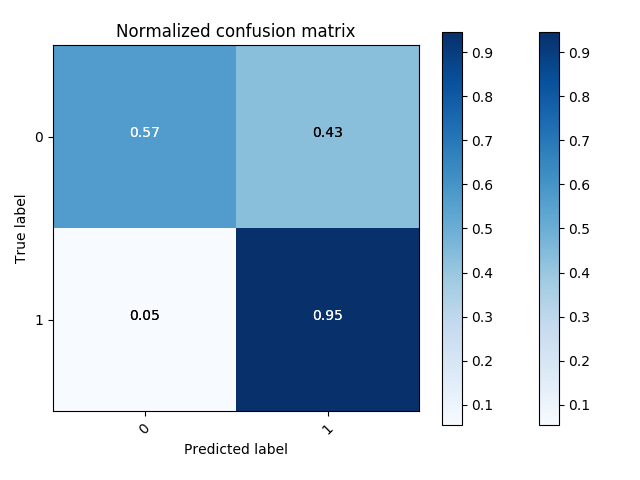
\includegraphics[width=0.4\textwidth]{img3.png}\label{fig:f1}}
		\hfill
		\subfloat[Confusion matrix for HMM]{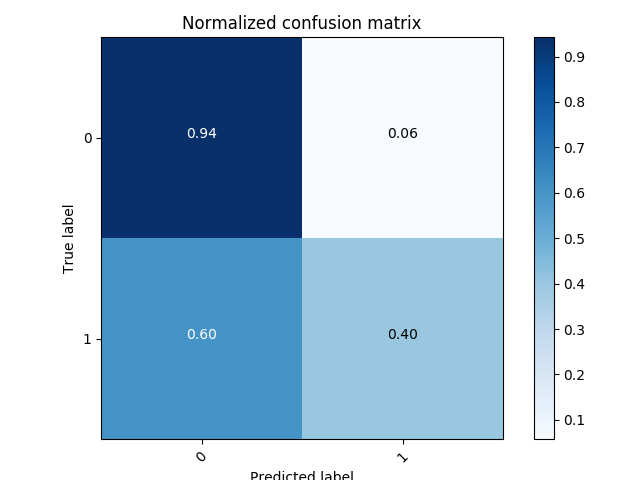
\includegraphics[width=0.4\textwidth]{img4.png}\label{fig:f2}}
		\caption{Confusion matrix for the HCRF and HMM models}
	\end{figure} 
	
	From the confusion matrix we can observe that for HCRFs the false positives are high whereas for HMMs the false negatives are high. Both the models have certain trade offs. 	
	
	\section{Conclusion}
	This report describes the solution approach to the following problems:
	\begin{enumerate}
	\item Given the genome information of a vaccinated person, determine whether the vaccine is effective or not
	\item Given the genome information of Plasmodium falciparum (or any other organism), determine the sequences which are antigenic.
	\end{enumerate} 
	
	The first problem can be solved with high accuracies. The gene sequence information of a person after vaccination is an effective indicator of whether the person will measurably benefit from the vaccine or not. This will enable us to hasten the process of testing vaccine effectiveness and reduce the time required for clinical trials.
	\\The second problem of identifying the target antigenic sequences from the genome sequence of Plasmodium falciparum is more challenging. Even complex sequential models using hidden states are not able to effectively capture the differences between antigenic and non antigenic sequences of Plasmodium falciparum. This is due to the nature of the genome sequence of Plasmodium falciparum. The differences between antigenic and non-antigenic sequences are subtle. The implications are that even better model which is the HMM model, in terms of accuracy, also has a high false negative rate.   
	\\Thus, we may reinforce the fact that developing a vaccine for malaria is challenging because of the nature of the genome sequence of its agent, Plasmodium falciparum. 
	
	\begin{thebibliography}{1}
		
		\bibitem{item0}
		http://www.who.int/mediacentre/factsheets/fs094/en/
		\bibitem{item01}
		https://www.cdc.gov/malaria/about/facts.html
		\bibitem{item02}
		http://www.who.int/malaria/areas/vaccine/en/
		\bibitem{item1} 
		https://www.historyofvaccines.org/content/articles/vaccine-development-testing-and-regulation
		\bibitem{item2}
		https://www.ncbi.nlm.nih.gov/geo/query/acc.cgi?acc=GSE18323
		\bibitem{item3}
		http://plasmodb.org/plasmo/
		\bibitem{item4}
		http://vaccine-safety-training.org/subunit-vaccines.html
		\bibitem{item5}
		S. B. Wang, A. Quattoni, L. Morency, D. Demirdjian, T. Darrell. Hidden Conditional Random Fields for Gesture Recognition. IEEE Computer Society Conference on Computer Vision and Pattern Recognition, 2006. 
		\bibitem{item6}
		D. L. Doolan, S. H. Apte, C. Proetti. Genome-based vaccine design: the promise for malaria and other infectious diseases. International Journal of Parasitology, 2014.
		\bibitem{item7}
		A.S. Kolaskar, P.C. Tongaonkar. A semi-empirical method for prediction of antigenic determinants on protein antigens. FEBS Letters, 1990.
		
	\end{thebibliography}
	
\end{document}